\documentclass{aruno-gist}

\usepackage{mylayout}

\webversionfalse

%% Details of the book
%% ===================

\title{Riflessioni sul Dhammapada}
\subtitle{52 strofe del Dhammapada con commenti di Ajahn Munindo}
\author{Ajahn Munindo}
\date{2017-07-25}
\editionInfo{\textit{Prima edizione}, 5.000 copie, prodotte in Malesia, 2018}
\ISBN{000-0-000000-00-0}% TODO ISBN

% \hyphenation{prep-a-ra-tion belief attrac-tive under-stand-ing moment}

\begin{document}

\ifwebversion
\webcover{%
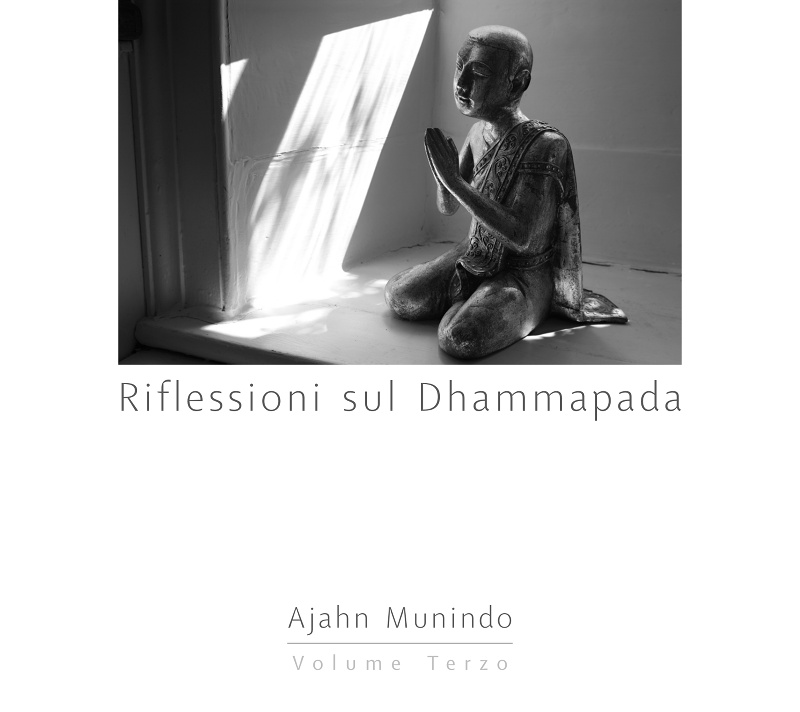
\includegraphics[width=\paperwidth]{./webcover.jpg}
}
\else

% Yellow color page
% Pantone 124M
% CMYK 0, 27, 100, 8

\thispagestyle{empty}
\mbox{}
\pagecolor{frontyellow}
\newpage
\thispagestyle{empty}
\pagecolor{white}
\mbox{}
\newpage

\fi

%% Frontmatter
%% ===========

\frontmatter*
\pagestyle{empty}

\midsloppy

\cleartorecto
\begin{quotepage}{60mm}
\centering
\itshape
Come un fiore\\
dal delizioso profumo\\
è la parola saggia e amorevole\\
accompagnata dalla retta azione.

{\smaller Dhammapada strofa 52}
\end{quotepage}



\cleartoverso
\begin{quotepage}{80mm}
\centering
\emph{Dedica}\\[0.4\baselineskip]
Vogliamo esprimere la nostra gratitudine per l’aiuto ricevuto da molte persone
nella preparazione di questo libro, in particolare al gruppo Kataññuta della
Malesia, Singapore e Australia, per averne reso possibile la stampa.

\end{quotepage}



\cleartorecto
\thispagestyle{empty}

\vspace*{1em}

{\centering

\soChapter{RIFLESSIONI SUL DHAMMAPADA}\\[0.4\baselineskip]
Volume 3
\vspace*{3\baselineskip}

{\itshape 52 strofe del Dhammapada\\
con commenti\\
di}

\vspace*{2\baselineskip}
Ajahn Munindo

\vfill

\soChapter{EDIZIONI SANTACITTARAMA}

}


\cleartoverso
\thispagestyle{empty}
\enlargethispage{\baselineskip}

{\copyrightsize\setlength{\parskip}{0.5\baselineskip}\setlength{\parindent}{0em}%
\raggedright%
\shaker\color[gray]{0.3}

\thetitle\\
di \theauthor

Traduzione di Chandra Candiani

Pubblicato da Edizioni Santacittarama, Monastero di Santacittarama,\\
02030 Poggio Nativo (RI), Italy

Titolo originale in inglese: Dhammapada Reflections

Pubblicato da Aruno Publications, Regno Unito (www.ratanagiri.org.uk)

Questo libro è scaricabile gratuitamente all'indirizzo\\
www.fsbooks.org e www.santacittarama.org

ISBN \theISBN

Copyright \copyright\ 2018 Associazione Santacittarama

\pali{Sabbadānaṃ dhammadānaṃ jinati}\\
``Il dono del Dhamma supera tutti i doni''

Foto di copertina di Gary Morrison

{\tiny
Quest'opera è distribuita con Licenza Creative Commons\\
Attribuzione - Non commerciale - Non opere derivate 4.0 Internazionale.\\
\href{http://creativecommons.org/licenses/by-nc-nd/4.0/deed.it}{http://creativecommons.org/licenses/by-nc-nd/4.0/deed.it}

Consultare pagina \pageref{copyright-details} per maggiori dettagli su diritti e restrizioni relativi a questa licenza.

Prodotto con \LaTeX\ typesetting system.

\theEditionInfo

}}



\chapterstyle{frontmatter}

\chapter{Prefazione}

{\centering
\emph{(Adattato dal Volume Uno)}% TODO confirm translation
\par}

\bigskip

\noindent
Da molto tempo, nei paesi buddhisti, è tradizione per i laici recarsi al
vicino monastero ogni luna nuova e luna piena per ascoltare un discorso
di Dhamma. In effetti, il Buddha stesso incoraggiò il suo Sangha a
mantenere questa pratica quindicinale. Anche se ora viviamo in un mondo
in cui le fasi della luna hanno meno significato, per molti è un aiuto a
rammentarsi dell'antica tradizione di cui facciamo parte.

Nel settembre del 2007 abbiamo iniziato a inviare versi del Dhammapada
scelti da `\emph{Dhammapada per la contemplazione}' del 2006. Veniva
offerta una strofa per ogni `giorno della luna', accompagnata da una
breve riflessione. Questo progetto è ora ben noto, si è diffuso
attraverso il passa-parola e le e-mail collettive. So che in varie parti
del mondo ci sono persone contente di ricevere un puntuale promemoria
dell'antica via, mentre affrontano la loro vita piena d'impegni. Altri
non vedono l'ora, ogni sera di luna nuova o di luna piena, quando
tornano dal lavoro, di aprire la casella di posta. Queste riflessioni
vengono usate in privato, riprodotte ampiamente, tradotte e fatte
girare. Ho anche sentito dire che fanno da base di discussione per gli
incontri dei gruppi settimanali di meditazione.

Era mia intenzione, condividendo in questo modo le mie personali
riflessioni, che magari anche altri si sentissero incoraggiati a mettere
in pratica la loro capacità riflessiva. C'è una tendenza, forse nei
praticanti buddhisti occidentali, a cercare di trovare la pace e la
comprensione fermando ogni forma di pensiero. Ma il Buddha ci dice che è
attraverso la `retta riflessione', che arriviamo a vedere la vera natura
della nostra mente; e non semplicemente fermando il pensiero.

Sono debitore nei confronti di molti che mi hanno aiutato nella
preparazione di questo materiale. Per i versi del Dhammapada ho
consultato varie autorevoli versioni. In particolare ho utilizzato il
lavoro del Venerabile Narada Thera (B.M.S. 1978), del Venerabile Ananda
Maitreya Thera (Lotsawa 1988), di Daw Mya Tin e gli editori della
Burmese Pitaka Association (1987) e di Ajahn Thanissaro. Per le storie
riportate insieme ai versi ho anche consultato
\href{http://www.tipitaka.net/}{www.tipitaka.net}.

\clearpage

Quando da più persone ho sentito dire che sarebbe stato utile
raccogliere in un libro queste riflessioni, mi sono rivolto al mio buon
amico Ron Lumsden. La sua notevole capacità di editing mi ha aiutato a
metter mano al mio lavoro per adattarlo a un numero maggiore di lettori.

Che le benedizioni che possono sorgere dalla compilazione di questo
volumetto siano condivise con tutti coloro che sono stati coinvolti
nella sua produzione e nel suo finanziamento. Che tutti quelli che
cercano la via possano trovarla e sperimentare alla fine la libertà. Che
tutti gli esseri possano cercare la via.

\bigskip

{\par\raggedleft
Bhikkhu Munindo\\
Monastero buddhista di Aruna Ratanagiri\\
Northumberland, Gran Bretagna\\
Stagione delle piogge (\emph{Vassa}) 2009
\par}


\chapter{Prefazione al Terzo Volume}

Queste strofe del Dhammapada e il loro commento sono il seguito del
primo e del secondo volume di questa serie. Come per gli altri volumi,
sono versioni leggermente riviste rispetto agli originali inviati alla
rete globale dei partecipanti a questa iniziativa. Se desiderate
ricevere le email direttamente ogni due settimane, potete iscrivervi a:

\bigskip

\noindent
https://ratanagiri.org.uk/teachings/dhammapada-reflections

\smallskip

\noindent
(per la versione originaria in inglese)

\bigskip

\noindent
http://santacittarama.altervista.org/subscribe.htm

\smallskip

\noindent
(per la versione tradotta in italiano)

\bigskip

{\par\raggedleft
Bhikkhu Munindo\\
Monastero buddhista di Aruna Ratanagiri\\
Northumberland, Gran Bretagna\\
Stagione delle piogge (\emph{Vassa}) 2015
\par}


%% Main matter
%% ===========

\mainmatter*

\cleartorecto
\thispagestyle{empty}
{\centering

\vspace*{0.6\textheight}
{\chapNameFont\LARGE\color{chaptitle}\soChapter{Riflessioni sul Dhammapada}}

}



\setcounter{chapter}{0}
\setcounter{page}{1}
\pagestyle{normalpage}
\chapterstyle{mainmatter}

\setlength{\parskip}{0.6\baselineskip}
\setlength{\parindent}{0pt}


%% == 1 ==

\begin{dhpVerse}{21}
\label{dhp-21}
La consapevolezza ricettiva apre alla vita\\
la fuga nella distrazione\\
è un sentiero di morte\\
chi è consapevole è totalmente vivo\\
chi è distratto\\
è come fosse già morto.
\end{dhpVerse}

\begin{dhpRefl}
  Il Buddha elogiava la coltivazione della consapevolezza. Ma, in un momento
  specifico, come riconoscere qual è il giusto oggetto di cui essere
  consapevoli? Le cose che vediamo, i suoni, gli odori, i sapori, le sensazioni
  tattili e le impressioni mentali sono così variegate. Possiamo semplicemente
  prestare attenzione alla natura mutevole, instabile di tutte le cose fintanto
  che iniziamo a vederle come inaffidabili e non veramente degne di
  attaccamento. Questo è essere consapevoli della peculiarità dei `contenuti'
  dell'esperienza. Cosa accade se applichiamo la consapevolezza al `contesto'
  dell'esperienza? La peculiarità del contesto in cui tutti gli oggetti
  dell'attenzione si manifestano è la stessa?
\end{dhpRefl}

%% == 2 ==

\begin{dhpVerse}{166}
\label{dhp-166}
Se conosci la tua strada\\
percorrila fino in fondo.\\
Non permettere alle richieste degli altri\\
per quanto insistenti\\
di distrarti.
\end{dhpVerse}

\begin{dhpRefl}
  Al primo sguardo, questi versi sembrano insegnare a non curarsi degli altri.
  Ma quel che il Buddha sottolinea è dove mettere il giusto accento nella nostra
  pratica. Se c’è carenza di ossigeno durante un volo, il pilota dice ai
  passeggeri di indossare prima la loro maschera e poi di aiutare gli altri. Non
  si invitano i genitori a non aiutare i figli ma a \emph{essere in grado} di
  aiutarli. Noi perdiamo facilmente il senso della prospettiva quando siamo
  sotto stress e agiamo in modi che peggiorano la situazione. Il Buddha vide
  quanto rapidamente le persone non risvegliate possano diventare distratte e
  confuse e così esortò i suoi monaci quando annunciò loro che stava morendo.
  Disse che chi gli era seriamente devoto non doveva preoccuparsi di portargli
  fiori; doveva invece intensificare il suo impegno nel praticare quanto aveva
  insegnato.
\end{dhpRefl}

%% == 3 ==

\begin{dhpVerse}{275}
\label{dhp-275}
Se segui il sentiero\\
arriverai alla fine della sofferenza.\\
Avendolo visto di persona\\
insegno la Via\\
che toglie tutte le spine.
\end{dhpVerse}

\begin{dhpRefl}
  La vita ferisce. La cosa più naturale è cercare un modo di stare in questo
  mondo che sia senza danno. Quelli che hanno percorso questa via prima di noi
  parlano dell'indescrivibile senso di sollievo nel raggiungere la terra della
  libertà. Ma aggiungono che è necessario uno sforzo abile. Il Buddha recitò
  questi versi a un gruppo di monaci che chiacchieravano di un viaggio fatto
  insieme. Egli spostò il discorso dalle strade e dai fiumi che avevano
  attraversato per portarlo sul terreno interiore. Il Maestro consiglia di usare
  il nostro tempo e la nostra energia limitati in un modo che ci portino nella
  direzione che più desideriamo seguire.
\end{dhpRefl}

%% == 4 ==

\begin{dhpVerse}{33}
\label{dhp-33}
Come il fabbro forgia una freccia\\
così il saggio trasforma la mente\\
di per sé irrequieta, instabile\\
e difficile da governare.
\end{dhpVerse}

\begin{dhpRefl}
  Allineare corpo e mente con quello che è vero, richiede una particolare
  abilità. Proprio quando pensavamo che la nostra pratica fosse valida, facciamo
  un passo falso e cadiamo di nuovo. Non importa se di tanto in tanto
  incespichiamo, è così che si impara a camminare, cadere ne è parte integrante.
  Quel che conta è sviluppare l'agilità e la prontezza a rimetterci in piedi e
  ricominciare da capo; senza guardare indietro.
\end{dhpRefl}

%% == 5 ==

\begin{dhpVerse}{418}
\label{dhp-418}
Chi smette\\
di contrapporre il mi piace al non mi piace\\
chi si è acquietato\\
chi non è influenzato\\
dalle condizioni del mondo\\
lo chiamo un grande essere.
\end{dhpVerse}

\begin{dhpRefl}
  Il mi piace e il non mi piace si succedono così rapidamente che sentiamo di
  non avere alcun controllo su di essi. Qualcuno ci dice qualcosa di piacevole e
  noi sentiamo che ci piace. Un altro ci dice qualcosa di offensivo e noi
  sentiamo che non ci piace. Può essere vero che non possiamo impedire
  l'emergere dei mi piace e non mi piace, ma se rallentiamo un po', possiamo
  notare che abbiamo una scelta; se seguirli o no, se costruire un `me' sulla
  loro base. Quando la consapevolezza è ben stabilizzata, i mi piace e i non mi
  piace possono essere visti come movimenti che si svolgono in una realtà più
  ampia. Cos'è quella realtà?
\end{dhpRefl}

%% == 6 ==

\begin{dhpVerse}{245}
\label{dhp-245}
Non è facile la vita di chi\\
conosce la vergogna,\\
è umile, puro di cuore\\
e distaccato, ha integrità\\
morale ed è riflessivo.
\end{dhpVerse}

\begin{dhpRefl}
  Se ci ritroviamo a pensare: ``Questo è troppo. Non
  posso lasciarlo andare'', dobbiamo essere ancora più attenti. È facile lasciar
  andare piccoli attaccamenti ma quelli davvero seri sono un'altra storia. Il
  Buddha conosceva quest'altra storia, quella in cui tendiamo a credere quando
  siamo di fronte ad attaccamenti profondi. La verità resta la verità per quanto
  possa essere dura, ogni sofferenza ha le sue radici nell'attaccamento, ed è la
  ragione per cui il Buddha ci ha dato insegnamenti come questo. È veramente
  difficile restare veri quando le forze dell'illusione ci trascinano. Che siano
  le influenze esterne degli oggetti sensoriali o le correnti interiori del
  condizionamento che ci dicono che siamo deboli e incapaci, risolutamente
  facciamo ritorno ai rifugi in cerca del potere per superare queste forze. Non
  si tratta semplicemente di sostituire a una storia negativa una positiva;
  chiediamo alla realtà di essere il nostro rifugio.
\end{dhpRefl}

%% == 7 ==

\begin{dhpVerse}{132}
\label{dhp-132}
Non far del male agli esseri viventi\\
che come noi cercano appagamento\\
significa far felici noi stessi.
\end{dhpVerse}

\begin{dhpRefl}
  Talvolta quello che facciamo porta alla felicità. Altre volte, quello che non
  facciamo porta alla felicità. Qui il Buddha dice che dovremmo essere
  consapevoli che lo sforzo di non far del male agli esseri viventi porta
  felicità non solo a chi vive libero da paura e sofferenza ma anche a noi. In
  un mondo in cui il nostro valore è spesso misurato in termini di produttività
  possiamo restare intrappolati nella sensazione di dover sempre fare qualcosa
  per migliorare le cose. Certe volte, il contenimento è la cosa più importante.
\end{dhpRefl}

%% == 8 ==

\begin{dhpVerse}{226}
\label{dhp-226}
Qualunque impurità viene mondata\\
nella mente di chi\\
sempre veglia,\\
giorno e notte educandosi\\
e dedicando tutta la sua vita\\
alla liberazione.
\end{dhpVerse}

\begin{dhpRefl}
  Se abbiamo fiducia nel sentiero e nella direzione in cui viaggiamo, non
  perderemo tempo in inutili vagabondaggi. Perciò gli insegnamenti ci
  incoraggiano a essere vigili. Tuttavia l'energia e la devozione verso la
  pratica spirituale non sono sufficienti. La nostra vita ha bisogno di essere
  diretta verso la giusta meta, sperimentando personalmente lo stato di perfetta
  libertà dalla sofferenza. Mentre percorriamo il sentiero, possiamo verificare
  se l'avanzamento e la direzione sono corretti osservando gli inquinanti della
  mente. Avidità, malevolenza, pigrizia, ansia, esitazione, stanno diminuendo o
  aumentando? Arriviamo a conoscere la realtà degli inquinanti non appena
  appaiono. E nello stesso modo, impareremo a vederli scomparire, qui e ora.
\end{dhpRefl}

%% == 9 ==

\begin{dhpVerse}{25}
\label{dhp-25}
Con l'impegno, l'attenzione\\
la rinuncia e la padronanza di sé\\
il saggio fa di se stesso un'isola\\
che nessuna inondazione può sommergere.
\end{dhpVerse}

\begin{dhpRefl}
  Certe volte sembra che il Buddha si contraddica. Ci insegna a coltivare la
  gentilezza amorevole verso tutti gli esseri, poi sembra dirci che dovremmo
  isolarci. Tutti gli insegnamenti del Buddha sono `indicazioni'; non sono
  posizioni fisse. Gli fu spesso chiesto di chiarire la sua posizione rispetto a
  una qualche visione filosofica. In tutti i casi, il Buddha cercò di evitare di
  dare a chi faceva la domanda una qualsiasi opinione a cui attaccarsi. Non si
  fissava su niente; si sintonizzava con il Dhamma nel suo manifestarsi. Il
  sentiero che ha insegnato è il \emph{Dhammavicaya}, l'investigazione della
  realtà. Diceva che ``non poteva altro che indicare la via'', sta a noi
  percorrere il cammino che ci ha mostrato.
\end{dhpRefl}

%% == 10 ==

\begin{dhpVerse}{236}
\label{dhp-236}
Affrettati a coltivare la saggezza.\\
Fai di te stesso un'isola.\\
Terso da macchie e imperfezioni\\
sarai un essere nobile.
\end{dhpVerse}

\begin{dhpRefl}
  Raggiungiamo lo stato di un essere nobile quando siamo una cosa sola con
  quello che veramente siamo. Il nostro lavoro consiste nel riconoscere quando
  diventiamo falsi, simulando di essere qualcosa o qualcuno che non siamo.
  Macchie e imperfezioni compaiono quando crediamo alle storie che ci racconta
  la mente. Se proviamo risentimento, abbiamo semplicemente bisogno di vedere
  con chiarezza la sensazione di risentimento. Se abbiamo paura, semplicemente
  abbiamo bisogno di vedere con chiarezza la sensazione di paura. Non abbiamo
  bisogno di fingere. Facciamo di noi stessi un'isola facendo della
  consapevolezza il fondamento della nostra vita. Questa consapevolezza che vede
  con chiarezza può indicarci la differenza tra il reale e il falso,
  conducendoci alla libertà.
\end{dhpRefl}

%% == 11 ==

\begin{dhpVerse}{65}
\label{dhp-65}
Come la lingua che gusta\\
il sapore della minestra\\
è chi vede distintamente\\
la verità, essendo stato un poco\\
in compagnia di chi è saggio.
\end{dhpVerse}

\begin{dhpRefl}
  Il numero di ritiri che facciamo non è importante quanto la nostra abilità di
  discernere la verità. La quantità di tempo che passiamo seduti a meditare non
  conta quanto la nostra capacità di vedere con chiarezza ciò che sta di fronte
  a noi. Se la nostra consapevolezza è qui e ora, dell'intero corpo-mente e
  priva di giudizio, possiamo allora imparare da ogni aspetto della nostra vita.
  Se abbiamo la fortuna d'incontrare la saggezza, in qualsiasi forma, la
  riconosceremo. Non deve sembrare buddhista, o all'avanguardia, e nemmeno
  apertamente saggia. Il cuore semplicemente la riconoscerà e ne sarà allietato.
\end{dhpRefl}

%% == 12 ==

\begin{dhpVerse}{198}
\label{dhp-198}
Restare liberi da angustia\\
anche in mezzo a chi si angustia\\
è vera felicità.
\end{dhpVerse}

\begin{dhpRefl}
  Quando le persone intorno a noi sono in difficoltà, potremmo sentire che in un
  certo senso non è giusto essere felici. Il Buddha ci dice l'opposto. La
  dimostrazione esteriore di una gioia eccessiva sarebbe fuori luogo, ma
  mantenere la gioia interiore è perfettamente adeguato. In effetti, può essere
  la cosa migliore da offrire in una situazione di turbamento.
\end{dhpRefl}

%% == 13 ==

\begin{dhpVerse}{399}
\label{dhp-399}
La forza della pazienza\\
è la risorsa degli esseri nobili:\\
possono venire incatenati,\\
sopportare attacchi fisici e verbali\\
senza abbandonarsi alla rabbia.
\end{dhpVerse}

\begin{dhpRefl}
  L'impulso moraleggiante dentro di noi va domato. Più siamo intelligenti, più
  dobbiamo essere cauti. Più la nostra parola è eloquente, più abbiamo bisogno
  di contenimento. Solo quando sappiamo di poter dire no a noi stessi, quando
  sappiamo di non dover sempre essere il vincitore possiamo apprezzare il potere
  trasformante della paziente tolleranza.
\end{dhpRefl}

%% == 14 ==

\begin{dhpVerse}{224}
\label{dhp-224}
Questi tre sentieri\\
portano tutti al paradiso:\\
dire la verità\\
non cedere alla rabbia\\
e dare, anche quando hai\\
ben poco da condividere.
\end{dhpVerse}

\begin{dhpRefl}
  Noi siamo i creatori del mondo. Le nostre azioni con il corpo, la parola, la
  mente danno forma allo spazio che abitiamo. Investire nella consapevolezza
  interiore ci libera dalla dipendenza dal mondo materiale. Le condizioni
  esterne della nostra vita vanno e vengono: a volte, sono piacevoli e
  gratificanti, altre, faticose e deludenti. Ma possiamo sempre fare lo sforzo
  di dire la verità. Possiamo sempre aspettare prima di soccombere alla rabbia.
  E al di là di quanto o quanto poco possediamo, possiamo sempre dare. Abbiamo
  già il potere di creare una bella dimora.
\end{dhpRefl}

%% == 15 ==

\begin{dhpVerse}{229-230}
\label{dhp-229}\label{dhp-230}
Chi vive in modo impeccabile\\
chi ha discernimento\\
è intelligente e virtuoso\\
viene apprezzato dal saggio.\\
Si può coprire di biasimo chi\\
nel suo essere è simile all'oro?\\
Anche gli dèi apprezzano il suo splendore.
\end{dhpVerse}

\begin{dhpRefl}
  A chi ci paragoniamo? L'abitudine mentale di paragonarci agli altri è per lo
  più espressione di confusione interiore che procura maggiore infelicità.
  Perché la radiosità del nostro vero essere risplenda liberamente, devono
  finire tutte le tendenze compulsive a paragonarci. Ma fintanto che soffriamo
  di questa abitudine, è meglio paragonarsi a chi vive impeccabilmente, a chi è
  più sveglio. Non ci è di aiuto avere in mente solo le immagini di chi ha più
  successo, è più ricco o più bello. Alcuni dei più grandi discepoli del Buddha
  non erano né famosi né belli, ma erano indubbiamente ammirati da tutti quelli
  che vedevano con limpidezza.
\end{dhpRefl}

%% == 16 ==

\begin{dhpVerse}{365-366}
\label{dhp-365}\label{dhp-366}
Lamentarsi della propria sorte\\
o invidiare i privilegi degli altri\\
ostacola la pace della mente.\\
Viceversa: contento\\
anche con poco\\
puro nel modo di vivere e vitale\\
sei da tutti tenuto in grande stima.
\end{dhpVerse}

\begin{dhpRefl}
  Questa semplice verità facilmente ci sfugge. Tristemente, siamo troppo
  propensi ad ammirare ed emulare chi non è particolarmente saggio. Qui, un
  Maestro molto saggio regge uno specchio e chiede: ``Vedi cosa stai facendo?
  Riesci a capire perché sei infelice?'' Non ci critica, né ci condanna, ma
  nemmeno ci lascia farla franca con le nostre abitudini. Con compassione, ci
  incoraggia a vedere le conseguenze della nostra inconsapevolezza. Talvolta ci
  sembra che ci sia sempre qualcosa di più da fare, qualcosa di più da ottenere,
  qualcos'altro di cui liberarsi. Anche la vita spirituale può apparire come un
  noioso tran tran. Ma credere sempre all'apparenza delle cose, non è la via
  verso la pace. Al posto dell'auto-commiserazione, può nascere la contentezza
  se siamo disposti a smettere di paragonarci sbadatamente agli altri.
\end{dhpRefl}

%% == 17 ==

\begin{dhpVerse}{271-272}
\label{dhp-271}\label{dhp-272}
Non accontentarti\\
di attenerti alle regole\\
e ai regolamenti\\
né di ottenere una vasta erudizione.\\
Non sentirti soddisfatto\\
perché raggiungi l'assorbimento meditativo\\
né perché dimori\\
in beata solitudine.\\
Dovresti essere contento\\
solo quando arrivi\\
al completo sradicamento\\
di ogni forma di ignoranza e inganno.
\end{dhpVerse}

\begin{dhpRefl}
  Leggere o ascoltare un insegnamento tanto profondo può far nascere una forte
  urgenza di praticare oppure l'impulso a rinunciare perché sentiamo di non
  farcela. Il modo in cui ci relazioniamo agli ideali determina se ne veniamo
  rafforzati o indeboliti. Gli ideali non ne sono di per sé responsabili. Quel
  che conta è che i nostri ideali siano in accordo con la Verità, ma è anche
  importante non scambiare un'immagine dell'obiettivo con l'obiettivo stesso. Il
  Buddha voleva che puntassimo alto; il più alto possibile e anche di più, ma
  non voleva che ci aggrappassimo all'ideale ignorando la nostra modestia.
  L'immagine dell'obiettivo dà la direzione come una bussola, e ovviamente non
  passiamo tutto il tempo a guardare la bussola. Fintantoché andiamo nella
  giusta direzione, pratichiamo con `questo', che è direttamente di fronte a
  noi.
\end{dhpRefl}

%% == 18 ==

\begin{dhpVerse}{352}
\label{dhp-352}
Maestro è chi ha abbandonato\\
ogni desiderio e ogni presa sul mondo\\
chi ha visto la verità\\
al di là delle forme eppure possiede\\
una profonda conoscenza delle parole.\\
Di tale grande essere si può dire\\
che abbia portato a compimento\\
il suo scopo.
\end{dhpVerse}

\begin{dhpRefl}
  Lasciar andare non è qualcosa che facciamo, è qualcosa che accade quando
  capiamo che quello che facciamo causa sofferenza. Finché siamo intrappolati
  nel cercare di lasciar andare, l'io che sta cercando di lasciar andare crea
  squilibrio. Ma anche non provarci affatto non è corretto. Cosa possiamo fare
  per realizzare il grande compito della ricerca della libertà? Che cosa
  significa fare un retto sforzo? Un aspetto del retto sforzo consiste
  nell'esaminare il tipo di sforzo che stiamo già facendo. Ci domandiamo: quello
  che facciamo è una forma di egocentrismo, o viene da un luogo più profondo,
  più quieto, un semplice interesse verso il vero? Sappiamo di voler essere
  liberi dalla sofferenza, ma è davvero utile il modo in cui lo vogliamo? Anche
  voler essere liberi può creare ostacoli se ci aggrappiamo a tale desiderio. La
  nostra aspirazione a `vedere la verità al di là delle forme' può essere di
  sostegno al retto sforzo, se rallentiamo, ci ricordiamo della gentilezza, ed
  esaminiamo come riceviamo l'esperienza del presente.
\end{dhpRefl}

%% == 19 ==

\begin{dhpVerse}{327}
\label{dhp-327}
Come un elefante con risolutezza\\
si trascina fuori da un pantano\\
elèvati con l'ispirazione\\
dell'attenzione coltivata.
\end{dhpVerse}

\begin{dhpRefl}
  L'energia dell'ispirazione può essere generata dalla saggia riflessione. Con
  il giusto tipo di sforzo, si possono affrontare le difficoltà insormontabili,
  si può sopportare l'insopportabile. L'ispirazione ha il potere di trasformare
  la nostra vita e il nostro mondo. Quando la saggia riflessione ci mostra che
  l'attenzione aiuta e la distrazione è di impedimento, il nostro cuore risponde
  volgendosi verso ciò che è salutare. L'equilibrata consapevolezza rivela in
  modo corretto l'entità del compito che abbiamo davanti a noi, con il nostro
  mondo interiore ostruito dall'ignoranza e il nostro mondo esteriore carico di
  ingiustizia. Però, la questione importante è: come affrontiamo questi compiti?
  Non è necessaria più forza, bensì una più attenta considerazione di causa ed
  effetto. Se a motivarci fossero chiara comprensione e gentilezza, il pantano
  dell'abitudine ad essere distratti apparirebbe meno avvilente. Una coltivata
  attenzione ci indica ciò che va bene, e la fiducia segue con naturalezza.
\end{dhpRefl}

%% == 20 ==

\begin{dhpVerse}{96}
\label{dhp-96}
Chi attraverso la retta comprensione\\
arriva allo stato\\
di perfetta libertà\\
è sereno nel corpo\\
nella parola, nella mente.\\
Gli alti e bassi della vita\\
non lo scuotono.
\end{dhpVerse}

\begin{dhpRefl}
  Il miglior modo per accogliere l'incertezza è attraverso la retta comprensione
  o retta visione. Sarebbe ingenuo aspettarsi di essere sempre a proprio agio
  con l'incertezza. Ma non dovremmo concludere di doverci assoggettare a essa.
  La vita, il cambiamento e tutto il resto che la concerne può sembrare
  `troppo', ma la vita di per sé non è mai troppo: è sempre `solo così'. Se la
  vita fosse davvero troppo, il Buddha non avrebbe mai potuto raggiungere la
  libertà mentre era ancora vivo. Quello che conta è la visione che abbiamo.
  Prendendoci troppo seriamente, la situazione può sembrare intollerabile,
  diventiamo tesi, e limitiamo le possibilità dell'intuizione profonda e della
  sensibilità. Rilassando il nostro modo di vedere, possiamo cercare di
  immaginare una realtà incondizionata in cui tutte le condizioni mutevoli
  appaiono sorgere e cessare. Il saggio lasciar andare porta a una
  consapevolezza espansa e a una prospettiva fresca su quanto facciamo e su come
  sia quello che facciamo a far sì che sembri che abbiamo un problema.
\end{dhpRefl}

%% == 21 ==

\begin{dhpVerse}{182}
\label{dhp-182}
Non è facile nascere\\
essere umano\\
e vivere una vita mortale.\\
Non è facile distinguere\\
la profonda saggezza\\
ma più raro di tutto\\
è che nasca un Buddha.
\end{dhpVerse}

\begin{dhpRefl}
  In termini di qui e ora, nasciamo come esseri umani ogni volta che abbiamo
  presenza mentale e integrità. A causa delle nostre tendenze a compromettere i
  principi del Dhamma, questo compito diventa difficile. È molto più facile
  seguire le nostre preferenze. Tuttavia, seguire semplicemente il mi piace e
  non mi piace non è vivere come potremmo vivere. Potremmo riflettere su causa
  ed effetto: cos'è accaduto l'ultima volta che mi sono perso nell'esperienza?
  In quest'epoca siamo fortunati ad avere un facile accesso al Dhamma, ma il
  Dhamma è difficile da udire perché abbiamo creato impedimenti avendo seguito
  le nostre preferenze così a lungo. Al tempo del Buddha, alcuni dei suoi
  discepoli si illuminavano sul momento, semplicemente ascoltando le sue parole.
  Perché non possiamo ascoltare nello stesso modo, comprendere il messaggio e
  lasciar andare il nostro carico? Se lo facessimo, il `Buddha' apparirebbe qui
  e ora.
\end{dhpRefl}

%% == 22 ==

\begin{dhpVerse}{43}
\label{dhp-43}
Non tua madre non tuo padre\\
né chiunque della famiglia\\
può darti dono più prezioso\\
di un cuore ben diretto.
\end{dhpVerse}

\begin{dhpRefl}
  Se il cuore è ben diretto, sentiamo che c'è qualcosa su cui possiamo fare
  affidamento quando le cose si fanno difficili. Se proviamo disperazione,
  delusione, disillusione, il cuore non deve sprofondare in un senso
  d'irreparabilità. Ma nemmeno deve cercare la sicurezza nella speranza. Il
  rifugio a cui affidarci non è affatto una cosa o uno stato; è una via. Avendo
  abbastanza a lungo esplorato le conseguenze dell'afferrarsi, ora cerchiamo la
  sicurezza nel lasciar andare le posizioni fisse. Abbiamo ancora opinioni e
  preferenze, ma non siamo così propensi a trovare in esse la sicurezza.
  Imparare a lasciar andare è la via per generare benedizioni.
\end{dhpRefl}

%% == 23 ==

\begin{dhpVerse}{276}
\label{dhp-276}
Il risvegliato\\
può solo indicare la via:\\
siamo noi a doverla percorrere.\\
Chi con saggezza riflette\\
e intraprende il sentiero\\
è libero dai ceppi di Mara.
\end{dhpVerse}

\begin{dhpRefl}
  ``Che sforzo dovrei fare? Dovrei fare qualcosa per questa situazione o
  semplicemente osservare la mente?'' Questi momenti di `non so' sono preziosi.
  L'incertezza non va considerata un fallimento. In effetti perdiamo qualcosa
  d'importante se abbiamo fretta di spingerli da parte. La realtà è che non so
  cosa fare e in questo non c'è necessariamente niente di sbagliato. Ma se sono
  completamente preso dall'impulso di sfuggire la sofferenza, perdo la verità
  della situazione, così com'è, e la possibilità di imparare da essa. Con la
  fiducia che nasce dal nostro impegno ai precetti possiamo permetterci di aver
  fiducia nell'essere pazienti e consapevoli del `non so', e delle sensazioni
  scomode che ne derivano. Sentite la forza dell'impulso a scappare dal `non
  so', a volerlo risolvere; rifiutate caparbiamente di esserne tirati in avanti.
  Possiamo provare ad aspettare finché la sensazione di essere spinti in avanti
  si placa e con calma ascoltiamo cosa l'intuizione ci suggerisca di fare.
\end{dhpRefl}

%% == 24 ==

\begin{dhpVerse}{297}
\label{dhp-297}
I discepoli del Buddha\\
sono pienamente svegli\\
giorno e notte\\
contemplando la realtà.
\end{dhpVerse}

\begin{dhpRefl}
  Il Buddha e i suoi discepoli realizzati si risvegliarono alla verità che stava
  proprio di fronte a loro. Come milioni di altri ricercatori, il futuro Buddha
  aveva cercato le risposte alle sue profonde domande nelle tecniche e nei
  sistemi di credenze. I rigori della rinuncia l'avevano portato quasi alla
  morte; ma niente di tutto questo aveva funzionato. Quello che invece aveva
  funzionato era stata la rinuncia a tutti gli sforzi di evitare la sofferenza,
  sia attraverso l'indulgenza al piacere che l'indulgenza al dolore, e aver
  preso l'esperienza stessa della sofferenza come suo maestro. Le Quattro Nobili
  Verità insegnate dal Buddha sono il suo modo per aiutarci a non perdere tempo.
  Egli voleva che i suoi discepoli si risvegliassero alla verità che esiste qui
  e ora, e scoprissero da sé la gioia e la chiarezza che vengono dalla Retta
  Comprensione.
\end{dhpRefl}

%% == 25 ==

\begin{dhpVerse}{374}
\label{dhp-374}
Quando i saggi dimorano\\
nella contemplazione\\
della natura impermanente\\
del corpo e della mente\\
e di tutta l'esistenza condizionata\\
provano gioia e contentezza\\
penetrando fino a ciò\\
che è intrinsecamente sicuro.
\end{dhpVerse}

\begin{dhpRefl}
  Tutti gli insegnamenti del Buddha indirizzano a ciò che è immutabile, che non
  muore, che è intrinsecamente soddisfacente. Ci soffermiamo nella
  contemplazione della natura che muta, che muore, insoddisfacente
  dell'esistenza condizionata per risvegliarci dal sogno in cui viviamo. Nel
  nostro mondo di sogno crediamo che attaccarci alle cose come se fossero
  fondamentali ci renderà felici. Il Buddha con il suo immediato accesso alla
  realtà incondizionata sapeva che aggrapparsi a qualsiasi aspetto della realtà
  condizionata è una via diretta alla delusione. E non lo insegnò perché
  creassimo una filosofia su come ogni cosa sia inaffidabile e deplorevole.
  Viveva in questo mondo come noi ma non soffriva e non si soffermava su quanto
  tutto questo sia triste. La vita può sembrare triste e deplorevole fin tanto
  che ci identifichiamo con il corpo-mente. L'identità del Buddha era
  indefinibile perché non si aggrappava a niente e la sua felicità era
  incrollabile perché non dipendeva da nulla.
\end{dhpRefl}

%% == 26 ==

\begin{dhpVerse}{185}
\label{dhp-185}
Non insultare, non maltrattare,\\
coltiva la rinuncia\\
nel rispetto della disciplina,\\
frugale nel mangiare e pago\\
della dimora che hai,\\
dònati all'intento consapevole:\\
questo è l'insegnamento del Buddha.
\end{dhpVerse}

\begin{dhpRefl}
  Essere frugali e contenti non fa parte della cultura del consumo. Ma fa parte
  della cultura buddhista. È vero che abbiamo bisogno di entusiasmo e di
  energia, di impegno e di concentrazione, se vogliamo raggiungere la meta della
  liberazione. Ma troppo di queste `virtù forti' non fa che crearci inutili
  ostacoli. Quando siamo consapevoli, abbiamo la possibilità di sapere se siamo
  fuori equilibrio e di modificarci di conseguenza. Le `virtù lievi' della
  contentezza, della frugalità, dell'umiltà sono meno attraenti per l'ego
  spirituale ma possono essere proprio quello di cui abbiamo bisogno per lasciar
  cadere il fardello.
\end{dhpRefl}

%% == 27 ==

\begin{dhpVerse}{329}
\label{dhp-329}
Ma se non trovi\\
un amico sincero\\
che coltiva integrità e saggezza\\
allora, come un re che lascia\\
una terra conquistata\\
o un elefante che vaga solitario nella foresta\\
procedi in solitudine.
\end{dhpVerse}

\begin{dhpRefl}
  L'integrità è la base della nostra pratica. Senza di essa nulla si sviluppa.
  Potremmo avere un parlare forbito e forse i nostri articoli potrebbero essere
  pubblicati nelle riviste, ma se manca l'integrità, la pratica non è mai
  iniziata. Percorrere il sentiero spirituale da soli non è un segno di
  fallimento; potrebbe essere addirittura l'opposto. Se le persone intorno a noi
  sono disposte a compromessi sulla impeccabilità, sarebbe meglio se fossimo da
  soli.
\end{dhpRefl}

%% == 28 ==

\begin{dhpVerse}{38}
\label{dhp-38}
In chi ha la mente instabile\\
il cuore non lavorato\\
dai veri insegnamenti\\
e una fede immatura\\
non è ancora cresciuta\\
appieno la saggezza.
\end{dhpVerse}

\begin{dhpRefl}
  Questa strofa del Dhammapada probabilmente descrive la situazione di quasi
  tutti noi: la mente serrata in modalità di pensiero, cresciuti con
  un'educazione spirituale minima e incapaci di dedicarci, con tutto il cuore, a
  qualcosa. Tuttavia abbiamo fiducia che la reale saggezza esista e che abbiamo
  la possibilità di realizzarla. È questo tipo `iniziale' di fede che ci fa
  cominciare e ci porta fin qui. Ora si tratta di costruire sulla sua base.
  Quando abbiamo provato il beneficio della pratica, la fede è `verificata' e si
  manifesta in modo assai diverso. Diventa un'affidabile fonte di energia.
  All'inizio eravamo motivati da un'idea o da un'intuizione. Ora l'invito è ad
  aver fiducia in una consapevolezza informata dall'esperienza. È come spendere
  soldi guadagnati con il nostro lavoro, anziché quelli che vengono da mamma e
  papà.
\end{dhpRefl}

%% == 29 ==

\begin{dhpVerse}{36}
\label{dhp-36}
La mente custodita e sorvegliata\\
fa sentire a casa.\\
Per quanto elusiva, sottile e difficile\\
da afferrare, chi è all'erta\\
dovrebbe custodire e sorvegliare la mente.
\end{dhpVerse}

\begin{dhpRefl}
  Quando custodiamo il nostro cuore-mente, coltiviamo la luce interiore. Quando
  la luce nel mondo esterno è tenue, siamo portati a sbagliarci riguardo alle
  cose. Magari scambiamo un pezzo di corda per un serpente e scappiamo presi da
  un panico assolutamente non necessario. Allo stesso modo, la mancanza di luce
  interiore ci spinge a reagire in modi folli, distruggendo il naturale senso di
  agio del nostro cuore. Non vedendo con chiarezza gli stari della mente,
  reagiamo e rendiamo peggiori le cose. Per esempio, forse ci sentiamo feriti
  per qualcosa successa anni fa e da allora continuiamo a rimuginare
  sull'amarezza perché non vediamo la verità della nostra reazione. Il perdono
  non è una virtù artificiale da passare sui nostri lividi. Anche se il ricordo
  di quello che è accaduto rimane, possiamo sempre scegliere se investire o meno
  di risentimento il ricordo. Questa pratica è sottile e difficile da capire ma
  vale il nostro sforzo.
\end{dhpRefl}

%% == 30 ==

\begin{dhpVerse}{248}
\label{dhp-248}
Chi dedica se stesso alla bontà\\
ricordi che è disastrosa\\
l'incapacità di dominarsi.\\
Non permettere\\
all'avidità e al comportamento scorretto\\
di prolungare la tua infelicità.
\end{dhpVerse}

\begin{dhpRefl}
  Il Buddha sa che la vita non è sempre facile. Sa che anche la pratica di
  osservare i precetti può essere difficile. La storia associata con questi
  versi coinvolge un gruppo di cinque discepoli laici, ciascuno dei quali
  osserva uno o due dei cinque precetti buddhisti. Ognuno di loro insiste che i
  suoi sono i più difficili da coltivare e perciò, per deduzione, i più
  meritevoli. Discutendo tra di loro, si avvicinano al Buddha. Ogni discepolo
  vuole che il Buddha lodi la sua pratica e sostenga il fatto che i precetti che
  il discepolo segue sono i più importanti. Invece, il Maestro li ammonisce,
  spiegando che nessuno dei cinque precetti è facile da mantenere, e nessuno di
  essi è meno importante e che tutti dovrebbero addestrarsi in tutti e cinque.
\end{dhpRefl}

%% == 31 ==

\begin{dhpVerse}{393}
\label{dhp-393}
Nessuno è da considerarsi\\
degno di rispetto\\
a causa della sua nascita o della sua cultura\\
o di qualsiasi altra qualità esteriore.\\
È la purezza\\
la comprensione della verità\\
che decide di qualcuno il merito.
\end{dhpVerse}

\begin{dhpRefl}
  Un essere liberato non si lascia mai ingannare dall'apparenza delle cose. Sa
  la differenza tra la `forma' esterna che gli occhi vedono e la `realtà' che il
  cuore conosce. Sente un naturale rispetto e un senso di piacere per
  l'intrinseca bellezza del `reale'. La nostra consapevolezza, tuttavia, è
  limitata a causa delle idee fisse e dobbiamo fare attenzione a non seguire
  casualmente il condizionamento della mente. Finché siamo inconsapevoli della
  verità, siamo suscettibili a restare colpiti dalle forme esterne. La bellezza
  transitoria, le intense emozioni, la ricchezza; tutto questo e altro ancora ci
  costringono a desideri inutili, per esempio vogliamo quello che non porta un
  beneficio durevole. Tutte le volte che mostriamo rispetto per la verità che è
  al di là della costrizione, accresciamo l'intimità con quella verità.
\end{dhpRefl}

%% == 32 ==

\begin{dhpVerse}{206}
\label{dhp-206}
È sempre un piacere\\
non avere a che fare con gli stolti.\\
Fa sempre bene incontrare\\
chi è nobile d'animo\\
ed è una gioia viverci insieme.
\end{dhpVerse}

\begin{dhpRefl}
  Il Buddha diede questo breve insegnamento riferendosi alle condizioni del
  mondo esterno, e non è difficile essere d'accordo. Possiamo anche contemplare
  lo spirito di questo messaggio in riferimento al mondo interiore; ai nostri
  stati mentali. Come ci sentiamo quando incontriamo pensieri stolti? Cosa
  succede quando smettiamo di indulgere in essi? Che effetto ha essere testimoni
  delle aspirazioni salutari del cuore? È possibile dimorare per lunghi periodi
  nelle intenzioni nobili?
\end{dhpRefl}

%% == 33 ==

\begin{dhpVerse}{212}
\label{dhp-212}
Prediligere è fonte di dolore.\\
Prediligere genera la paura di perdere.\\
Se invece sei libero dalla predilezione\\
non c'è dolore,\\
e come potrebbe esserci paura?
\end{dhpVerse}

\begin{dhpRefl}
  Una possibile lettura di questo testo è che è sbagliato avere a cuore le cose:
  la famiglia, gli amici, i ricordi. Questa interpretazione letterale incolpa i
  sentimenti in se stessi della nostra sofferenza. Ma il Buddha non sta parlando
  solo dei sentimenti, sta mostrandoci come poter essere liberi. È possibile
  sentire predilezione e allo stesso tempo essere liberi? Quando seppe che i
  suoi due principali discepoli, i Venerabili Sariputta e Mogallana, erano
  morti, il Buddha commentò che era come se il sole e la luna se ne fossero
  andati dal cielo. Non sembra proprio una persona che non sentisse niente.
  Conoscere la verità dei sentimenti significa che non troviamo più la nostra
  identità nei sentimenti. Lasciarli andare non significa che scompaiano. In
  cosa tutti questi sentimenti sorgono e svaniscono? Quella è la dimora del
  Buddha, perciò egli poteva sentire pienamente e liberamente, senza sofferenza.
\end{dhpRefl}

%% == 34 ==

\begin{dhpVerse}{100}
\label{dhp-100}
Una sola parola vera\\
che acquieta la mente\\
è meglio di mille\\
futili parole.
\end{dhpVerse}

\begin{dhpRefl}
  Ascoltare ore di discorsi di Dhamma può essere utile, ma il Buddha dice che
  una sola parola può essere sufficiente. Quello che conta è che quella parola
  tocchi veramente il nostro cuore. Vi sembra vero? La verità è quello che ci
  cura, non le parole. Vivendo in un mondo distratto dal materialismo, spesso
  pensiamo che di più è meglio. Ma un piccolo assegno di un milione di euro vale
  molto di più di un grosso camion carico di vecchi giornali. Si tratta in
  entrambi i casi di carta. Qual è la differenza? Già sappiamo che è necessario
  badare alla qualità, non solo alla quantità. Questa strofa del Dhammapada ci
  incoraggia a portare questa comprensione più in profondità.
\end{dhpRefl}

%% == 35 ==

\begin{dhpVerse}{183}
\label{dhp-183}
Smetti di fare il male\\
coltiva il bene\\
purifica il cuore.\\
È questa la Via\\
del Risvegliato.
\end{dhpVerse}

\begin{dhpRefl}
  Il primo stadio della coltivazione dell'integrità consiste nell'astenersi dal
  seguire ciò che è male. Consiste nel dire `no' a noi stessi quando è
  necessario. Come risultato, scopriamo più tardi di poter dire `sì' senza
  perdere noi stessi. Se non riconosciamo i nostri impulsi malsani per quello
  che sono, possiamo pensare che le cose brutte siano solo negli altri. Il
  secondo stadio della coltivazione dell'integrità consiste nello sviluppare ciò
  che è buono. Anche se si tratta solo di un breve momento di bontà, non
  scartatelo. Il terzo stadio consiste nel purificare il nostro sforzo dalla
  macchia dell'`io'. Anche quando abbiamo completamente terminato di ridipingere
  una stanza, l'odore delle esalazioni della pittura resta. Sebbene la nostra
  pratica possa farsi più forte, potrebbe rinforzarsi anche il senso
  dell'auto-importanza.
\end{dhpRefl}

%% == 36 ==

\begin{dhpVerse}{205}
\label{dhp-205}
Gustando il sapore della solitudine\\
e il nettare della pace\\
chi beve della gioia\\
che è la sostanza della realtà\\
vive libero dalla paura del male.
\end{dhpVerse}

\begin{dhpRefl}
  I medici ci consigliano di nutrire il corpo nutrendoci in modo sano e facendo
  regolarmente esercizio fisico. Il Buddha ci consiglia di nutrire il cuore con
  la Verità. Se ci lasciamo sommergere dagli impegni, dimentichiamo quanto ci
  ringiovanisca passare del tempo da soli; riservare del tempo per se stessi.
  Una sensazione di scontentezza gradualmente cresce finché finiamo per credere
  di mancare intrinsecamente di qualcosa. Questa percezione può far comodo alla
  cultura del consumo, ma non ci dà forza interiore. Talvolta la pratica
  spirituale implica avere il coraggio di afferrare meno e aver fiducia nello
  stato naturale, incontaminato del nostro cuore.
\end{dhpRefl}

%% == 37 ==

\begin{dhpVerse}{197}
\label{dhp-197}
Restare liberi dall'odio\\
anche in mezzo a chi odia\\
è vera felicità.
\end{dhpVerse}

\begin{dhpRefl}
  Di solito, noi identifichiamo la felicità con l'ottenere quello che vogliamo.
  Esistono altre forme di felicità? Tutti attraversiamo periodi in cui non
  abbiamo quello che vogliamo, o abbiamo quello che assolutamente non vogliamo.
  In questa strofa il Buddha indica una qualità di felicità che non dipende
  dall'ottenere o meno quello che vogliamo; una felicità che proviene dalla
  saggezza. La saggezza sa che alcune condizioni possono essere cambiate e altre
  no. Per esempio, non possiamo impedire a qualcun altro di provare odio. Ma
  possiamo compiere lo sforzo per non essere tirati dentro la sua rabbia. E
  nonostante quel che si possa dire, questo non è immobilismo. È prendersi la
  responsabilità per quanto è nostro e mantenere l'equanimità verso quello che
  non lo è.
\end{dhpRefl}

%% == 38 ==

\begin{dhpVerse}{391}
\label{dhp-391}
Chi si astiene dal provocare sofferenza\\
attraverso il corpo, la parola e la mente\\
è chiamato un grande essere.
\end{dhpVerse}

\begin{dhpRefl}
  La grandezza può essere definita in termini di influenza sociale che abbiamo o
  di beni che possediamo, ma nella mente del Buddha è piuttosto determinata da
  come le persone si comportano. Questo è un modo molto pratico per valutare
  quanto degna di fiducia sia una persona. Si contiene nel suo modo di agire e
  di parlare? È gentile? Non possiamo dire quello che le succede interiormente,
  ma possiamo osservare l'effetto che ha sul mondo intorno a lei.
\end{dhpRefl}

%% == 39 ==

\begin{dhpVerse}{7}
\label{dhp-7}
Come un vento burrascoso\\
sradica un albero fragile\\
così chi incurante si aggrappa al piacere\\
indulge al cibo e alla pigrizia\\
può sradicarlo Mara.
\end{dhpVerse}

\begin{dhpRefl}
  Come conoscere la giusta quantità? I nostri sensi e la società ci dicono
  spesso che abbiamo bisogno di più. L'economia globale è basata sul
  condizionarci a credere che siamo mancanti di qualcosa. Se il nostro rifugio è
  in una consapevolezza espansa, priva dell'abitudine compulsiva a prendere
  posizioni, siamo nella situazione di poter contemplare il processo del
  condizionamento. È essenziale riconoscere che non dobbiamo essere asserviti al
  nostro ambiente. Il lavoro della riflessione interiore può condurre a una
  fiducia indipendente dalla credenza collettiva o dalla tendenza culturale.
  Possiamo sperimentare il non mangiare in eccesso o il non avere un'opinione su
  qualsiasi cosa. Possiamo starcene bene quieti e coltivando la contentezza. La
  contentezza non significa abdicazione. Quello che conta è, quando scoppia un
  temporale, veniamo travolti? Da dove prendiamo la nostra forza?
\end{dhpRefl}

%% == 40 ==

\begin{dhpVerse}{164}
\label{dhp-164}
Come il bambù distrugge se stesso\\
nel dare frutto\\
a se stessi fanno male gli stolti\\
prestando fede a false opinioni\\
e deridendo i saggi\\
che vivono in accordo con la Via.
\end{dhpVerse}

\begin{dhpRefl}
  È facile criticare le debolezze degli altri. È difficile riconoscere e sanare
  gli errori dentro di sé. A un certo livello, può anche far sentire bene
  elevare se stessi buttando giù gli altri, ma simili sentimenti non sono
  affidabili. Essere sempre in vantaggio sugli altri è improbabile che
  contribuisca all'armonia. Ovviamente, ci sono momenti in cui la critica è
  necessaria, ma perché sia costruttiva ci vuole un'intenzione salutare.
  Conoscere con accuratezza la propria intenzione significa probabilmente dover
  rallentare un po', aspettare e ascoltare dentro di sé prima di parlare.
\end{dhpRefl}

%% == 41 ==

\begin{dhpVerse}{42}
\label{dhp-42}
Peggio di un ladro\\
peggio di un nemico\\
un cuore mal indirizzato\\
invoglia a nuocere.
\end{dhpVerse}

\begin{dhpRefl}
  Un cuore mal indirizzato ci porta a nuocere quando ostacola l'accesso allo
  stato naturale della contentezza. Quando la consapevolezza fallisce e ci
  attacchiamo, l'atto dell'aggrapparsi alimenta il pensiero confuso e l'azione
  che divide. Il benessere vero, che esiste autonomamente, sorge senza sforzo
  per chi è uno con ciò che è; con il Dhamma. Un essere liberato non deve
  cercare di essere contento o cercare di non essere scontento. Avendo visto la
  sofferenza causata dall'aggrapparsi, ogni tendenza ad attaccarsi a posizioni
  fisse se n'è andata. Il cuore non ostacolato porta solo alla comprensione e
  all'agio.
\end{dhpRefl}

%% == 42 ==

\begin{dhpVerse}{15}
\label{dhp-15}
Quando con chiarezza vediamo\\
la nostra mancanza di virtù\\
il rimorso ci assale;\\
sia ora che in futuro ci affliggiamo.
\end{dhpVerse}

\begin{dhpRefl}
  Se sbattessimo un dito del piede e non sentissimo male, saremmo nei guai. Il
  dolore è un messaggio che dice: ``Fai attenzione.'' Se dovessimo agire o
  parlare con crudeltà senza sentire rimorso, ugualmente saremmo nei guai. In
  che altro modo potremmo imparare? Nonostante le apparenze, il rimorso non è
  qualcosa di sbagliato. È lì per proteggerci; una sorta di sistema immunitario.
  Possiamo ascoltarlo, accettarlo, accogliere il dolore nel nostro cuore perché
  ci insegni a non seguire più in futuro la trascuratezza. Perdersi nel rimorso
  porta al senso di colpa; e abbiamo perso anche il punto. Non impariamo
  compiacendoci a odiare noi stessi o gli altri per aver sbagliato.
\end{dhpRefl}

%% == 43 ==

\begin{dhpVerse}{131}
\label{dhp-131}
Far male agli esseri viventi\\
che come noi cercano appagamento\\
significa far male a noi stessi.
\end{dhpVerse}

\begin{dhpRefl}
  L'interesse verso se stessi può essere utilizzato per la nostra ricerca della
  retta azione. Di fronte al pericolo ci sentiamo subito minacciati, i nostri
  cuori si infiammano e il saggio discernimento si oscura. Tuttavia, invece di
  perderci in una reazione difensiva, la retta formazione può aiutarci a
  ricordare che siamo `tutti nella stessa barca'. Noi tutti condividiamo il
  desiderio di essere liberi dalla sofferenza. Probabilmente l'aggressore ha
  dimenticato questo fatto, da qui il suo intento a farci del male; ma fino a
  quando saremo anche noi intenzionati a fargli del male, solo un aumento della
  reciproca sofferenza ne conseguirà. Rammentare regolarmente l'universalità
  della sofferenza può proteggerci dal cadere in questo vortice. Dedicare
  quotidianamente un breve periodo di tempo a considerare come siamo tutti alla
  ricerca di appagamento, può dar luogo allo svilupparsi di sentimenti di
  empatia e compassione. Questo non è un argomento di cui saremo convinti
  tramite il solo ragionamento, ma se ci immergiamo in tale contemplazione
  potremo noi stessi trovarne beneficio.
\end{dhpRefl}

%% == 44 ==

\begin{dhpVerse}{123}
\label{dhp-123}
Come vigile e protettivo\\
rimane colui cui si affida\\
un carico prezioso\\
evita il male come un veleno.
\end{dhpVerse}

\begin{dhpRefl}
  Noi abbiamo una merce preziosa: la coscienza umana. E amiamo la vita; da qui,
  lo sforzo che mettiamo nel proteggerla. Il Buddha sta dicendo che dovremmo
  sorvegliare la fortuna ereditata evitando tutte le cattive azioni. Possiamo
  trovare un grande beneficio in questa vita se siamo attenti e coltiviamo la
  saggezza. Allo stesso modo, una grande sofferenza può derivare se siamo
  disattenti. `Male' è una parola forte e magari preferiamo non usarla. Ma
  saremo ingenui se non la prendessimo in considerazione. Quando il cuore è
  posseduto dall'avidità o dall'odio, ne possono conseguire azioni malvagie. Una
  volta compiute, ne deriveranno conseguenze dolorose. Nessuno può salvarci
  dalla disattenzione, nemmeno il Buddha. Con la gentilezza e la saggia
  riflessione contribuiamo alla protezione di tutti gli esseri.
\end{dhpRefl}

%% == 45 ==

\begin{dhpVerse}{408}
\label{dhp-408}
Grande è colui\\
che dice la verità\\
che offre delicato incoraggiamento\\
che non polemizza con nessuno.
\end{dhpVerse}

\begin{dhpRefl}
  Ci sono momenti in cui è necessario essere assertivi. Come assertivo è il
  sistema immunitario del nostro corpo quando affronta una malattia. Ma non
  facciamo dell'assertività il nostro unico modo d'essere. Può apparire forte,
  notevole, ma ha i suoi limiti. Ci sono momenti in cui è la delicatezza a
  essere richiesta. Anche la parola gentile, se è vera e incoraggiante, produce
  risultati.
\end{dhpRefl}

%% == 46 ==

\begin{dhpVerse}{318}
\label{dhp-318}
Opinioni distorte\\
che additano come giusto ciò che è sbagliato\\
e sbagliato ciò che è giusto\\
portano gli esseri alla disgregazione.
\end{dhpVerse}

\begin{dhpRefl}
  Talvolta è necessario ricordarci che le cause della sofferenza, la nostra e
  quella del mondo, sono complesse. Spesso, non è quello che accade nel mondo
  esterno a determinare le nostre lotte, ma il modo in cui vediamo le cose. Non
  è saggio ritenere validi punti di vista e opinioni solo perché sono
  comunemente sostenuti. Forse è conveniente, ma non è una buona ragione per
  investire in essi. È semplicistico colludere con il pensiero collettivo senza
  esaminarne le conseguenze. Avere delle preferenze è naturale, ma attaccarvisi
  e costruire un'identità nel sostenerle porta al pregiudizio e alla
  disgregazione, interiormente ed esteriormente.
\end{dhpRefl}

%% == 47 ==

\begin{dhpVerse}{291}
\label{dhp-291}
Fallisci\\
nella ricerca della felicità\\
se è alle spese\\
dell'altrui benessere.\\
Ti intrappola ancora\\
il laccio della malevolenza.
\end{dhpVerse}

\begin{dhpRefl}
  La felicità è come il cibo: ci nutre. Ma tuttavia perché sia salutare e
  autenticamente nutriente, i nostri sforzi devono essere accompagnati da
  empatia. È miope lottare per essere felici, senza però consapevolezza di come
  turbiamo gli altri. Forse pensiamo di generare cause di benessere, ma coviamo
  nel cuore gelosia o inimicizia.
\end{dhpRefl}

%% == 48 ==

\begin{dhpVerse}{151}
\label{dhp-151}
Tramandato dai saggi\\
è il sapere che la verità\\
sopravvive alla dissoluzione\\
benché ciò che è esternamente\\
entusiasmante\\
perda di smalto\\
e benché il corpo decada.
\end{dhpVerse}

\begin{dhpRefl}
  Non solo i nostri corpi ma tutti gli oggetti materiali sono soggetti alla
  legge dell'impermanenza; come pure le strutture sociali, le istituzioni, le
  relazioni, e le organizzazioni. Tutto ciò che sta intorno e dentro a noi è in
  uno stato di perenne flusso. Da bambini, per uno sviluppo equilibrato, è
  necessario essere in qualche modo protetti da questo dato di fatto. Per
  esempio, non ricordiamo costantemente ai bambini la mortalità della mamma e
  del papà. Ma quando cresciamo, presto o tardi, dobbiamo ammettere che questa è
  la realtà così com'è. In effetti, più che ammetterlo abbiamo bisogno di
  accogliere questa verità, se vogliamo saggiamente accordarci con la
  mutevolezza delle condizioni. Il Buddha considerò la legge dell'impermanenza
  come qualcosa al di là della degenerazione; qualcosa di stabile e di sicuro;
  una Verità a cui possiamo rivolgerci, per trovare un sistema di riferimento.
\end{dhpRefl}

%% == 49 ==

\begin{dhpVerse}{129}
\label{dhp-129}
Provando empatia per gli altri\\
si scopre che tutti gli esseri hanno paura\\
della punizione e della morte.\\
Allora, non si assale\\
né si provoca più nessuno.
\end{dhpVerse}

\begin{dhpRefl}
  L'empatia è l'essenza dell'armonia. Nel corso della nostra vita dipendiamo a
  vari livelli dagli altri. Se dimentichiamo che tutti noi desideriamo la
  felicità e temiamo il dolore, rischiamo di essere dominati da preoccupazioni
  auto-centrate. Possiamo però imparare a riconoscere quello che ci accomuna.
  L'empatia sostiene l'intuizione profonda dell'altruismo. Attraverso l'empatia
  capiamo che, come noi, anche gli altri sperano di non venire delusi e anche
  gli altri temono di perdere le cose che gli sono care. Anche il desiderio di
  fare del male a qualcun altro è una forma di sofferenza che condividiamo con
  gli altri. Tutti coloro il cui senso d'identità proviene dall'attaccamento al
  loro corpo-mente sono costretti a persistere nella disarmonia, nei pensieri e
  sensazioni distorti che ne conseguono. Lasciar andare l'attaccamento a questo
  corpo-mente e riconoscere la nostra identità nella comprensione, significa che
  la disarmonia semplicemente non sorgerà.
\end{dhpRefl}

%% == 50 ==

\begin{dhpVerse}{92}
\label{dhp-92}
Come gli uccelli non lasciano\\
orme nell'aria\\
la sua mente non si aggrappa\\
alle tentazioni che gli si offrono.\\
La sua rotta\\
è lo stato di liberazione senza tracce\\
invisibile agli altri.
\end{dhpVerse}

\begin{dhpRefl}
  Possiamo fare quello che facciamo così completamente, così pienamente, da non
  lasciarci dietro alcuna orma? Probabilmente no. La nostra abitudine ad
  aggrapparci significa che tendiamo a fare le cose in modo parziale. La nostra
  parola può essere manipolatoria, e lasciarsi dietro un senso di incertezza. Le
  nostre azioni possono essere egoistiche e lasciare dietro di sé un senso di
  incompletezza. E i nostri pensieri possono essere sparsi dappertutto,
  lasciandoci confusi. Questa immagine delicata degli uccelli che volano nel
  cielo, senza lasciare dietro di sé alcuna orma, ci invita a vivere senza
  attaccamento. Nel compiere questo sforzo, ci allineiamo ai grandi esseri che
  hanno fatto quanto andava fatto, lasciandosi dietro nient'altro che la Verità.
\end{dhpRefl}

%% == 51 ==

\begin{dhpVerse}{296}
\label{dhp-296}
I discepoli del Buddha\\
sono pienamente svegli\\
giorno e notte\\
contemplando il Risvegliato.
\end{dhpVerse}

\begin{dhpRefl}
  Possiamo ammirare il nostro Maestro, il Buddha, senza rinunciare a chi e cosa
  siamo in questo preciso momento. Alcuni, quando sono invitati alla
  contemplazione del Maestro spirituale, tradiscono se stessi nel tentativo di
  imitare un altro. Il Buddha non voleva che ignorassimo chi sentiamo di essere
  e fingessimo di essere un altro; incoraggiava piuttosto una ricettività con
  cuore aperto e mente chiara di `questa' persona, qui e ora, inclusi tutti i
  nostri limiti e ossessioni. Assumere un nuovo insieme di abitudini
  condizionate nel tentativo di essere liberi dalla sofferenza non è
  liberazione, è abdicazione. Nella pratica, includiamo tutto di noi stessi in
  un vasto campo di consapevolezza, libera da discriminazione e pregiudizio, e
  così facendo offriamo tutto di noi stessi al servizio del Dhamma.
\end{dhpRefl}

%% == 52 ==

\begin{dhpVerse}{285}
\label{dhp-285}
Recidi i vincoli d'affetto\\
come si coglie un fiore d'autunno.\\
Percorri il sentiero della liberazione\\
esposto dal Risvegliato.
\end{dhpVerse}

\begin{dhpRefl}
  Non ci libereremo dagli attaccamenti aggrappandoci a opinioni su come dovrebbe
  essere la vita. E qui con `vita' si intende tutto: se stessi, gli altri, i
  possessi materiali. Anche le opinioni religiose procurano sofferenza se le
  prendiamo nel modo sbagliato. Si tratta invece di riconoscere, nel momento
  stesso in cui lo facciamo, come ci aggrappiamo alle cose. Perché opponiamo
  resistenza alla realtà del cambiamento? Il cambiamento è costante ma noi non
  lo vediamo. Percorrere la Via del Risvegliato verso la liberazione significa
  esaminare la nostra relazione con qualsiasi esperienza, piacevole o spiacevole
  che sia. Ogni singolo momento della nostra vita è un'opportunità per imparare
  come lasciar andare, lasciar essere e comprendere.
\end{dhpRefl}



\backmatter

\bookmarksetup{startatroot}

\chapterstyle{backmatter}
\newgeometry{vmargin=15mm, hmargin=10mm}

% FIXME: remove page number before index page

\chapter{Indice dei Primi Versi}

{\smaller
\setlength{\parskip}{0pt}
\setlength{\parindent}{0pt}

\begin{longtable}[c]{llr}
s. 7 & Come un vento burrascoso & \pageref{dhp-7}\\
s. 15 & Quando con chiarezza vediamo & \pageref{dhp-15}\\
s. 21 & La consapevolezza ricettiva apre alla vita & \pageref{dhp-21}\\
s. 25 & Con l'impegno, l'attenzione & \pageref{dhp-25}\\
s. 33 & Come il fabbro forgia una freccia & \pageref{dhp-33}\\
s. 36 & La mente custodita e sorvegliata & \pageref{dhp-36}\\
s. 38 & In chi ha la mente instabile & \pageref{dhp-38}\\
s. 42 & Peggio di un ladro & \pageref{dhp-42}\\
s. 43 & Non tua madre non tuo padre & \pageref{dhp-43}\\
s. 65 & Come la lingua che gusta & \pageref{dhp-65}\\
s. 92 & Come gli uccelli non lasciano & \pageref{dhp-92}\\
s. 96 & Chi attraverso la retta comprensione & \pageref{dhp-96}\\
s. 100 & Una sola parola vera & \pageref{dhp-100}\\
s. 123 & Come vigile e protettivo & \pageref{dhp-123}\\
s. 129 & Provando empatia per gli altri & \pageref{dhp-129}\\
s. 131 & Far male agli esseri viventi & \pageref{dhp-131}\\
s. 132 & Non far del male agli esseri viventi & \pageref{dhp-132}\\
s. 151 & Tramandato dai saggi & \pageref{dhp-151}\\
s. 164 & Come il bambù distrugge se stesso & \pageref{dhp-164}\\
s. 166 & Se conosci la tua strada & \pageref{dhp-166}\\
s. 182 & Non è facile nascere & \pageref{dhp-182}\\
s. 183 & Smetti di fare il male & \pageref{dhp-183}\\
s. 185 & Non insultare, non maltrattare, & \pageref{dhp-185}\\
s. 197 & Restare liberi dall'odio & \pageref{dhp-197}\\
s. 198 & Restare liberi da angustia & \pageref{dhp-198}\\
s. 205 & Gustando il sapore della solitudine & \pageref{dhp-205}\\
s. 206 & È sempre un piacere & \pageref{dhp-206}\\
s. 212 & Prediligere è fonte di dolore. & \pageref{dhp-212}\\
s. 224 & Questi tre sentieri & \pageref{dhp-224}\\
s. 226 & Qualunque impurità viene mondata & \pageref{dhp-226}\\
s. 229-230 & Chi vive in modo impeccabile & \pageref{dhp-229}\\
s. 236 & Affrettati a coltivare la saggezza. & \pageref{dhp-236}\\
s. 245 & Non è facile la vita di chi & \pageref{dhp-245}\\
s. 248 & Chi dedica se stesso alla bontà & \pageref{dhp-248}\\
s. 271-272 & Non accontentarti & \pageref{dhp-271}\\
s. 275 & Se segui il sentiero & \pageref{dhp-275}\\
s. 276 & Il risvegliato & \pageref{dhp-276}\\
s. 285 & Recidi i vincoli d'affetto & \pageref{dhp-285}\\
s. 291 & Fallisci & \pageref{dhp-291}\\
s. 296 & I discepoli del Buddha & \pageref{dhp-296}\\
s. 297 & I discepoli del Buddha & \pageref{dhp-297}\\
s. 318 & Opinioni distorte & \pageref{dhp-318}\\
s. 327 & Come un elefante con risolutezza & \pageref{dhp-327}\\
s. 329 & Ma se non trovi & \pageref{dhp-329}\\
s. 352 & Maestro è chi ha abbandonato & \pageref{dhp-352}\\
s. 365-366 & Lamentarsi della propria sorte & \pageref{dhp-365}\\
s. 374 & Quando i saggi dimorano & \pageref{dhp-374}\\
s. 391 & Chi si astiene dal provocare sofferenza & \pageref{dhp-391}\\
s. 393 & Nessuno è da considerarsi & \pageref{dhp-393}\\
s. 399 & La forza della pazienza & \pageref{dhp-399}\\
s. 408 & Grande è colui & \pageref{dhp-408}\\
s. 418 & Chi smette & \pageref{dhp-418}\\
\end{longtable}

}



%% Gift of Dhamma
%% --------------

\cleartorecto
\thispagestyle{plain}
{\smaller\centering

\emph{“Il dono del Dhamma supera ogni altro dono”}

Questo libro è offerto per la distribuzione gratuita, nella\\
speranza che possa essere di beneficio a chi desidera\\
intraprendere un cammino di approfondimento e\\
comprensione del proprio vivere. Per noi del monastero\\
Santacittarama è un grande privilegio rendere disponibili\\
libri come questo, e saremmo felici di continuare a farlo.

Riceviamo volentieri i commenti e le osservazioni dei lettori.\\
I costi di questa pubblicazione sono stati coperti da libere\\
donazioni – una preziosa opportunità per molti di\\
sponsorizzare iniziative e dedicare la propria offerta, in linea\\
con la tradizione buddhista. Future ristampe di questa o di\\
altre opere dello stesso genere dipendono direttamente dai\\
contributi offerti in tal senso. Chi fosse interessato a\\
partecipare alla sponsorizzazione di “Doni di Dhamma” come\\
questo, può contattarci al seguente indirizzo:

MONASTERO SANTACITTARAMA\\
Località Brulla, 02030 Poggio Nativo (Rieti)\\
www.santacittarama.org\\
sangha@santacittarama.org

}


%% Copyright details
%% -----------------

\cleartoverso
\thispagestyle{plain}
\vspace*{-2.5\baselineskip}
\enlargethispage{\baselineskip}

{\copyrightsize\setlength{\parindent}{0pt}%
\raggedright\label{copyright-details}
\setlength{\parskip}{3pt}
{\centering

{\large\ccbyncnd}

Quest'opera è distribuita con Licenza Creative Commons\\
Attribuzione - Non commerciale - Non opere derivate 4.0 Internazionale.\\
\href{http://creativecommons.org/licenses/by-nc-nd/4.0/deed.it}{http://creativecommons.org/licenses/by-nc-nd/4.0/deed.it}

}

Tu sei libero di:
\begin{packeditemize}
  \item Condividere -- riprodurre, distribuire, comunicare al pubblico, esporre in pubblico, rappresentare, eseguire e recitare questo materiale con qualsiasi mezzo e formato
\end{packeditemize}

Alle seguenti condizioni:

\begin{packeditemize}
\item Attribuzione -- Devi riconoscere una menzione di paternità adeguata.
\item NonCommerciale -- Non puoi utilizzare il materiale per scopi commerciali.
\item Non opere derivate -- Se remixi, trasformi il materiale o ti basi su di esso, non puoi distribuire il materiale così modificato.
\end{packeditemize}

Note:

Non sei tenuto a rispettare i termini della licenza per quelle componenti del
materiale che siano in pubblico dominio o nei casi in cui il tuo utilizzo sia
consentito da una eccezione o limitazione prevista dalla legge.

Non sono fornite garanzie. La licenza può non conferirti tutte le autorizzazioni
necessarie per l'utilizzo che ti prefiggi. Ad esempio, diritti di terzi come i
diritti all'immagine, alla riservatezza e i diritti morali potrebbero
restringere gli usi che ti prefiggi sul materiale.

{\centering
  \color[gray]{0.4}\rule{0.4\linewidth}{0.1pt}%
\par}

Harnham Buddhist Monastery Trust operating as Aruno Publications asserts its moral right to be identified as the author of this book.

Harnham Buddhist Monastery Trust requests that you attribute ownership of the work to Aruno Publications on copying, distribution, display or performance of the work.

}


\end{document}